\section{Обработка данных}
	В результате вычислений, которые заняли примерно месяц, были полученные $.dat$ файлы. Каждый из этих массивов данных соответствует определённому временному шагу. Для последующей обработки и на их основе построение графиков использовалось встроенное средство ANSYS CFD-Post. Для анализа влияния вихрегенераторов на локальное трение и перенос использовались различные сечения в разных частях канала. Некоторые из них представлены на рисунке \ref{fig:planesforanalysis}. 
	\begin{figure}[H]
		\centering
		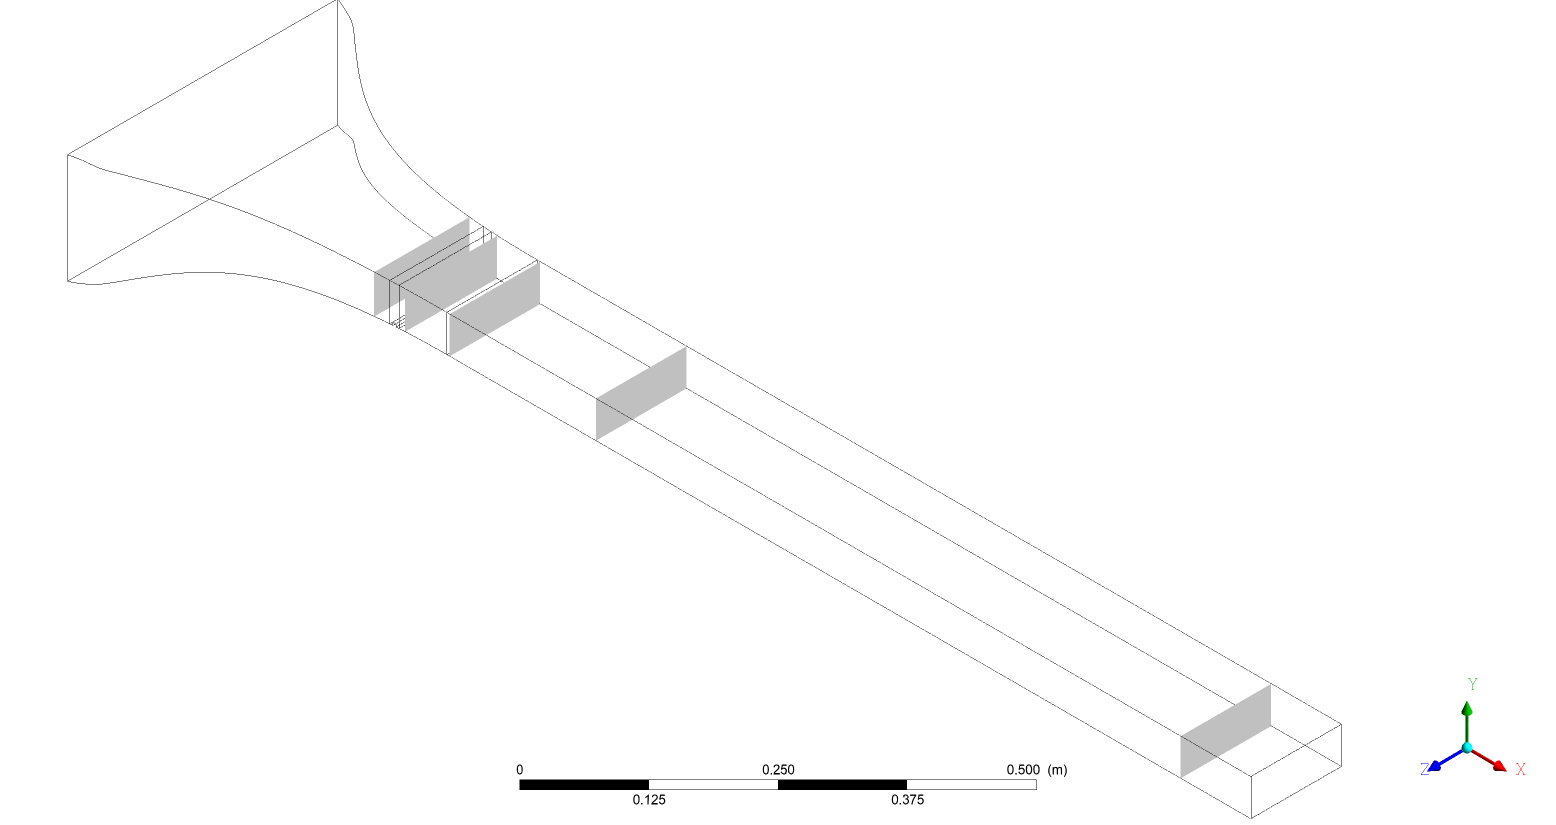
\includegraphics[width=0.9\linewidth]{../Assets/1}
		\caption{Сечения для анализа}
		\label{fig:planesforanalysis}
	\end{figure}
	
	Начало координатный осей модели расположено в центре входа канала. Рассматривались сечения на разных высотах вдоль и различных расстояниях от входа в канал. На таблице ниже представлен перечень сечений, расположение и их описание. Изображения в приложениях имеют названия исходя из таблицы. % ??? по человечески написать ??? %
	\begin{table}[H]
		\begin{center}
			\begin{tabular}{|c|c|c|c|}
				\hline
				Подпись & Плоскость & Расположение & Описание\\
				\hline
				PlaneXY & XY & Z = 0 & вдоль всего канала\\
				\hline
				PlaneYZ300 & YZ & X = 300 & перед препятствием\\
				\hline
				PlaneYZ340 & YZ & X = 340 & за проволокой\\
				\hline
				PlaneYZ400 & YZ & X = 400 & на входе в прямой участок\\
				\hline
				PlaneYZ600 & YZ & X = 600 & далее по каналу\\
				\hline
				PlaneYZ1400 & YZ & X = 1400 & на выходе из канала\\
				\hline
				PlaneXZ0 & XZ & Y = 0 & над пограничным слоем\\
				\hline
				PlaneXZ20M & XZ & Y = -20 & над препятствием\\
				\hline
				PlaneXZ23М & XZ & Y = -23 & на уровне проволоки\\
				\hline
			\end{tabular}
		\end{center}
		\label{tbl:sections}
		\caption{Перечень сечений}
	\end{table}
\section{Влияние на локальное трение и перенос}
\subsection{Скорость}
\subsection{Трение}
\subsection{Напряжение}